\section{Goals}

Our goal in this thesis was to create machine learning models for three different tasks:

\begin{itemize}
  \item Classify whether a participant belongs to the \textbf{control} group or \textbf{condition} group.
  \item Classify a participant's depression class (by MADRS score).
  \item Predict a participant's MADRS score.
\end{itemize}

The models were going to be One-Dimensional Convolutional Neural Networks. We solved all these using each participant's activity data as input, and we created a model that, with few changes, could be used for all three goals. For the different goals, only the last few layers needed to change. 

For the first goal, classifying \textbf{control} or \textbf{condition} group, the output data was a matrix with two columns (\textbf{control}, \textbf{condition}), with a $1$ in one of the columns and a $0$ in the other for each row. 

However, first, we wanted to see if these problems were solvable with simple regression. The idea was to throw in the columns from the demographics dataset \ref{figure:demographics}. We did not expect much from this, as there are only 55 rows in the table. Anyone having a little bit of experience with machine learning will know that this is not nearly enough data. However, we wanted to do it regardless, and see how a simple and stupid model performed. Doing this, we established some benchmark for performance; the Convolutional Neural Network model had to \textit{at least} better than this one.

\subsection{Learning experiments}

We needed to learn more about convolutional neural networks, so we proceeded to implement an image recognition algorithm. We found a tutorial on how to make a 2D CNN for classifying cats and dogs from images \cite{2d_cnn} and thought it would be an excellent way to learn.

It was both a fun and informative experience in implementing this. Especially when we extended the script to allow an image URL to predict on, we could browse for images of cats and dogs on the Internet, and find out if the model could classify them (in most cases it did). We even tried inputting images of humans to the model for fun, to see if they looked more like a dog or a cat.

However as mentioned before, the activity measurements are of one dimension, so we could not use this network.

\begin{quote}
  \textit{A 1D CNN is very effective when you expect to derive interesting features from shorter (fixed-length) segments of the overall dataset and where the location of the feature within the segment is not of high relevance. This applies well to the analysis of time sequences of sensor data (such as data from gyroscopes or accelerometers).} \cite{1d_cnn}
\end{quote}

To learn more about one-dimensional convolutional neural networks, we followed a tutorial \cite{1d_cnn}, which used a dataset containing accelerometer data from a smartphone on the participant's waists. The goal here was to predict what a given person is doing at the time, given the accelerometer data for that time slice. What the given person is doing is one of the following:

\begin{itemize}
  \item Standing
  \item Walking
  \item Jogging
  \item Sitting
  \item Upstairs
  \item Downstairs
\end{itemize}

As we followed the tutorial and implemented the model, we learned a lot about how one-dimensional convolutional neural networks work and how we should structure our data to make it work for our dataset.

We also got some ideas about where our dataset could provide more data. What if the dataset containing the current mental state of the bipolar patient? Then someone could make some automated system that always can tell a patient whether they are not depressed, manic or depressive. However data collection for this kind of task would be difficult because we cannot always know what the patient thinks, nor does the patient. The tutorial dataset is different because it is easy to differentiate physical states of the body like standing or walking.

\section{Preparing Input Data}

\subsection{Input data}

As we said before, we wanted the input data to be the same for each goal, since we wanted to use a similar model on all three.
The tutorial \cite{1d_cnn} sliced up the measurements with overlap, and labeled the slices. We also did this.

We created a list where for each participant in the demographics table \ref{figure:demographics}, measurements for $N$ hours were grouped. 
Another choice we learned from the tutorial was to overlap the sequences, so we made the next group of $N$ hours start \textit{$M$} hours after, 
and not \textit{$N$} hours after the group before, as one might think. When this list was complete with sequences from all participants, we 
had to \textbf{reshape} it so that it could fit into a neural network. We ended up with a feature list (which we called \textbf{segments}), 
where each element was a list of activity measurements for 4 hours: 

\textbf{segments[0] = [[0], [143], [0], [20], [166], [160], [306], [277], [439], ...]}

\subsection{Output data}

A second list was created simultaneously, where the value here was different for each goal. 

\subsubsection{Classifying participant group}

For classifying control/condition group, this list was built to contain the values \textbf{0} or \textbf{1} for the labels \textbf{[CONTROL]} and \textbf{[CONDITION]}, which was chosen according to the group the participants were in. Using a helper function from Keras, \textbf{to\_categorical}, we transformed this list of labels into the matrix we described. We had to transform the values to a categorical matrix in order to be able to select a \textit{category} for classification. This list, which we called \textbf{labels}, looked like this: 

\textbf{labels[i] = [0, 1]}

\noindent Meaning that segment $i$ is labeled as \textbf{[CONDITION]}.

\subsubsection{Depression Classes}
Here we wanted to classify which depression class a participant belonged to, and as described in the earlier, we divide MADRS scores into some cutoff-points, which we used as \textit{classes} in our classification:

\begin{itemize}
  \item 0-6: normal
  \item 7-19: mild depression
  \item 20-34: moderate depression
  \item 34-60: severe depression
\end{itemize}

So instead of labelling the segments as \textbf{[CONTROL]} or \textbf{[CONDITION]}, we labeled them as 0, 1 or 2 (we ignored 3 as there are no participants with MADRS scores this high). One element in \textbf{labels} after making it a categorical matrix looked like this:

\textbf{labels[i] = [0, 1, 0]}

\noindent Meaning that segment $i$ is labelled as \textbf{[MILD DEPRESSION]}.

\subsubsection{Predicting MADRS Score}

Instead of classifying one of three or one of two classes which we have done earlier, this time we wanted to predict the actual MADRS score value. Creating the output data for this goal is easier; we appended the MADRS score for the corresponding participant to the list. For example:

\textbf{scores[i] = [18]}

\section{Performance Metrics}

When finishing with a training session for a machine learning model, we need to use different metrics to be able to tell how the model performed based on some testing data. For prediction models, we only consider the loss, but evaluating classification models happens differently. 

To begin with, we will focus on one performance metric which is called accuracy. This one makes sense to the human brain; telling a friend that has no experience in machine learning or data science that we have made our computer able to classify something with 98\% accuracy is something that they would understand. Other metrics include \textit{confusion matrix}, \textit{precision}, \textit{Recall}, \textit{specificity} and \textit{F1 score}, which will be described below.

\subsection{Confusion Matrix}

\begin{figure}[h]
  \begin{center}
    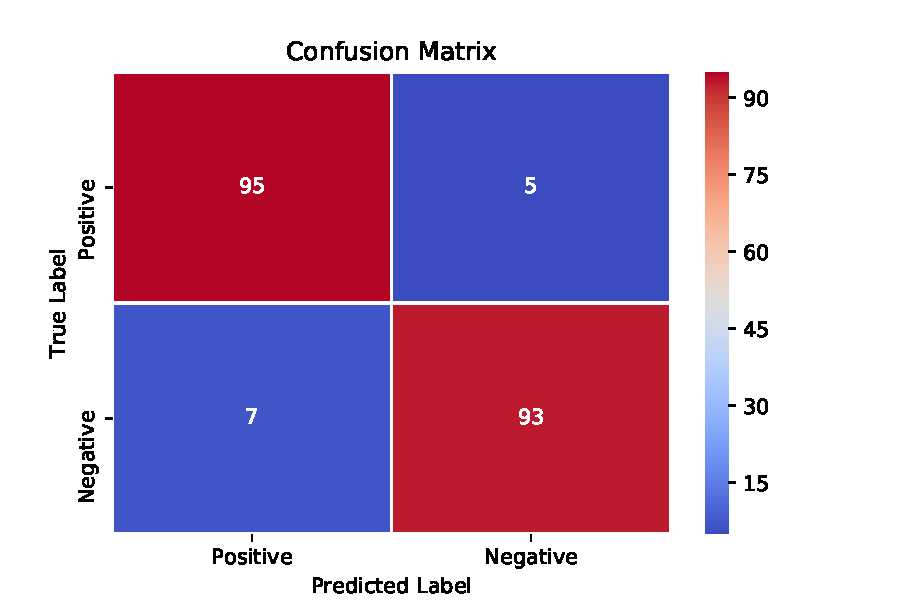
\includegraphics[height=8cm]{img/conf_matrix.pdf}
    \caption{Confusion Matrix Example}
    \label{figure:confusion_matrix_bipolar}
  \end{center}
\end{figure}

Figure \ref{figure:confusion_matrix_bipolar} shows a \textit{confusion matrix}. It is a visual metric for classification models in machine learning and is the basis for the other performance metrics. It can tell how well our model is performing by having correlation values for the different classes. Let us say we have 200 samples in our test data to use on our model that classifies control vs. condition group. 

A \textit{confusion matrix} for a good model would look like figure \ref{figure:confusion_matrix_bipolar}, with high numbers in \textbf{True Positive} and \textbf{True Negative} and as low numbers as possible in \textbf{False Positive} and \textbf{False Negative}. Having a high number in \textbf{True Positive} means that the model can classify that a participant is in the condition group if he or she is, and having a high number in \textbf{True Negative} means that the model can classify that a participant is in the control group if this is the case. The other cases, \textbf{False Positive} and \textbf{False Negative}, is where the model made a wrong classification, and therefore as close these numbers are to zero the better our model is.

\subsection{Accuracy}

\blockquote[\cite{ml_metrics}]{Accuracy is a good measure when the target variable classes in the data are nearly balanced.}

When calculating the \textit{accuracy}, we sum up the correct predictions and divide that with the total number of predictions ($ \frac{TP + TN}{TP + TN + FN + FP} $). For our example (\ref{figure:confusion_matrix_bipolar}), the \textit{accuracy} would be $ \frac{93 + 95}{93 + 95 + 5 + 7} = 94\% $. It is a good metric to use for our example because the number of samples for each variable class is well balanced ($ 93+5=98 $ samples where \textbf{condition group} was the correct option, and $ 7+95=102 $ samples where \textbf{control group} was correct).

Terrible use of the \textit{accuracy} metric would be when one of the classes strongly dominates the samples. For example, if a model predicts \textbf{cancer} vs. \textbf{no cancer}, and the samples contain five people with cancer, and the 95 remaining people do not. The model would be terrible at predicting cancer and still have an accuracy score of $ 95\% $ \cite{ml_metrics}.

\subsection{Precision} 

Precision operates entirely on the predicted positives, and it tells us how many \textbf{true positives} there is among \textbf{predicted positives} ($ \frac{TP}{TP + FP} $) \cite{ml_metrics}. 

This performance metric is better to use on \textit{unbalanced} classes than accuracy. The \textit{cancer vs no cancer} example, assuming it predicts no-one to have \textbf{cancer}, would yield a precision score of $ \frac{5}{5+95} = 5\% $. And our \textit{control vs condition} example would result in a precision score of $ \frac{93}{93+7} = 93\% $.

\subsection{Recall}

\textit{Recall} is another useful performance metric. It tells us the relationship between \textbf{true positives} and \textbf{actual positives}, for example how many participants classified to be in the condition group there were among total participants in the condition group.

The calculation of recall is done by dividing \textbf{true positives} by \textbf{true positives + false negatives} ($ \frac{TP}{TP+FN} $), which translates into $ \frac{93}{93+5} \approx 95\% $ (using the confusion matrix) \ref{figure:confusion_matrix_bipolar}.

Choosing a metric to use from \textit{precision} or \textit{recall} depends on your goal. Try to achieve close to $ 100\% $ \textit{recall} if you want to reduce \textbf{false negatives}, and likewise with \textit{precision} if you want to reduce \textbf{false positives} \cite{ml_metrics}.

\subsection{Specificity}

As \textit{recall} operates on \textbf{actual positives}, \textit{specificity} is the exact opposite metric. It tells us the relationship between \textbf{true negatives} and \textbf{actual negatives}. So if your goal is to reduce \textbf{false positives}, specificity is a valid choice. \textit{Specificity} is calculated by dividing \textbf{true negatives} by \textbf{true negatives + false positives} ($ \frac{TN}{TN+FP} $). For the confusion matrix \ref{figure:confusion_matrix_bipolar}, the \textit{specificity} score equals $ \frac{95}{95+7} \approx 93\% $.

\subsection{F1 Score}

The metrics that we have described in this section are all useful when determining whether our classification model is good enough. However, the relationship between \textit{recall} and \textit{precision} and knowing when to use which can be confusing, at least if the different classes are somewhere between entirely unbalanced and perfectly balanced (for example a 35\% split). 

Therefore another metric called \textit{F1 Score} was created, which gives us a balanced value combining \textit{recall (R)} and \textit{precision (P)}. The basic idea is to return the \textit{mean} value of the two scores (F1 = $ \frac{P + R}{2} $), but that would not be balanced if one score is much lower than the other. F1 score actually uses something called \textit{harmonic mean} instead of the standard \textit{arithmetic mean}, and is calculated as $ 2 \cdot \frac{P \cdot R}{P + R} $ \cite{ml_metrics}. 
Following this formula, the F1 score for confusion matrix \ref{figure:confusion_matrix_bipolar} becomes:

\[
  F1 = 2 \cdot \frac{P \cdot R}{P + R} = 2 \cdot \frac{0,93 \cdot 0,95}{0,93 + 0,95} \approx 94\%
\]

\subsection{Classification Report}

A machine learning framework for Python, \textit{sklearn}, includes a package with functions to calculate most of these scores. Just import and use them like this: 

\begin{figure}
\begin{code}
  \begin{minted}[linenos]{python}
    from sklearn.metrics import confusion_matrix, 
                                precision_score, 
                                recall_score, 
                                f1_score, 
                                classification_report

    # ... set up model, make predictions ...

    print(confusion_matrix(y, y_class_predicted))
    print(precision_score(y, y_class_predicted))
    print(recall_score(y, y_class_predicted))
    print(f1_score(y, y_class_predicted))
    print(classification_report(y, y_class_predicted))
  \end{minted}
  \caption{Metric score functions from sklearn.}
  \label{code:sklearn_metrics}
\end{code}
\end{figure}

\begin{table}[h]
\begin{center}
  \begin{tabular}{| l | l | l | l | l |}
    \hline
                  & precision & recall  & f1-score & support \\ \hline
    class 0       & 0.05      & 1.00    & 0.67     & 1       \\
    class 1       & 0.00      & 0.00    & 0.00     & 1       \\
    class 2       & 1.00      & 0.67    & 0.80     & 3       \\
                  &           &         &          &         \\ 
    micro avg     & 0.60      & 0.60    & 0.60     & 5       \\
    macro avg     & 0.50      & 0.56    & 0.49     & 5       \\
    weighted avg  & 0.60      & 0.60    & 0.60     & 5       \\
    \hline
  \end{tabular}
  \caption{\textit{Classification Report from sklearn. It shows precision, recall and F1-score for each class.}}
  \label{table:classification_report}
\end{center}
\end{table}

The classification report returns a matrix (see table \ref{table:classification_report}) with \textit{precision}, \textit{recall}, \textit{F1 score} and another column called \textit{support} (simply how many samples of data there are for this class). The rows describe each class used for prediction \cite{sklearn_classification_report}.